
% --------------------------------------------------------------- CONFIGURATIONS

%ifdef TWOSIDE
	%\documentclass[a4paper,12pt,final,twoside,openright]{book}
%elif ONESIDE
	\documentclass[a4paper,12pt,final,oneside]{book}
%endif

\usepackage{rapport}


% -------------------------------------------------------------- META: CONSTANTS

\newcommand{\reporttitle}{ERP}
\newcommand{\enseignants}{Youssef~\textsc{Amghar}\\ Anne~\textsc{Legait}\\ Pierre-Alain~\textsc{Millet}\\ Mohamed~\textsc{Ouhalima}}
\newcommand{\reportauthor}{Guillaume~\textsc{Abadie}\\ Thierry~\textsc{Cantenot}\\ Marina~\textsc{Julien}\\ Ahmed~\textsc{Kachkach}\\ Martin~\textsc{Wetterwald}\\ Valentina~\textsc{Zantedeschi}}
\newcommand{\hexanome}{SpecIFic}
\newcommand{\reportsubject}{Livrable de projet}
\newcommand{\stagetopic}{Blablabla test}
\newcommand{\dateperiod}{du 17 décembre 2013 au 11 mars 2014}
\newcommand{\HRule}{\rule{\linewidth}{0.5mm}}
\setlength{\parskip}{1ex} % Espace entre les paragraphes

\hypersetup{
	pdftitle={\reporttitle},%
		pdfauthor={\reportauthor},%
		pdfsubject={\reportsubject},%
		pdfkeywords={INSA Lyon}
}

\title{\reporttitle}
\author{\reportauthor}
%\setcounter{tocdepth}{4}


% ------------------------------------------------------------------------- FILE

\begin{document}


    % ------------------------------------------------------------------- HEADER

	\renewcommand{\chaptername}{} %\renewcommand{\thechapter}{}
	\renewcommand{\contentsname}{Sommaire}

	\pagestyle{empty}
	\pagenumbering{Roman}


    % ------------------------------------------------------------ HEADER: TITLE

	% Inspiré de http://en.wikibooks.org/wiki/LaTeX/Title_Creation
\begin{center}
	\begin{minipage}[t]{0.48\textwidth}
	  \begin{flushleft}
	    
\includegraphics [width=40mm]{images/logo_INSA.png} \\[0.5cm]
			INSA Lyon\\
			20, avenue Albert Einstein\\
			69621 Villeurbanne Cedex
	  \end{flushleft}
	\end{minipage}
	\begin{minipage}[t]{0.48\textwidth}
	  \begin{flushright}
	    %\includegraphics [width=60mm]{images/logo_Passau.jpg} \\[0.5cm]
	    %Universität Passau\\
		%Innstraße, 3\\
		%	D-94032 Passau
	  \end{flushright}
	\end{minipage} \\[2cm]

	\textsc{\Large \reportsubject}\\[0.3cm]
	\HRule \\[0.4cm]
	{\Huge \bfseries \reporttitle}\\[0.3cm]
	{\LARGE \bfseries «~\stagetopic~»}\\[0.3cm]
	{\Large \dateperiod}\\[0.4cm]
	\HRule \\[1cm]

	
\includegraphics [scale=0.35]{images/i7.jpg} \\[0.7cm]
	\begin{minipage}[t]{0.4\textwidth}
	  \begin{flushleft} \large
	    \emph{Hexanôme \textbf{\hexanome}~:}\\
	    \small \reportauthor
	  \end{flushleft}
	\end{minipage}
	\begin{minipage}[t]{0.5\textwidth}
	  \begin{flushright} \large
	    \emph{Enseignants~:} \\
	    \enseignants
	  \end{flushright}
	\end{minipage}

	\vfill
	\footnotesize{Année scolaire 2013-2014}
\end{center}


	%ifdef TWOSIDE
		%\cleardoublepage
	%endif

	%\include{title2}

	%ifdef TWOSIDE
		%  \newpage
		%	\null
		%	\vfill
	%endif


    % --------------------------------------------------- HEADER: CONFIGURATIONS

	\sloppy          % Justification moins stricte : des mots ne dépasseront pas des paragraphes

    \frontmatter
		\pagestyle{empty}
		\tableofcontents
		\addtocontents{toc}{\protect\thispagestyle{empty}}

	\mainmatter
	\pagestyle{headings}

	\renewcommand{\thechapter}{\Alph{chapter}}
	\renewcommand{\chaptermark}[1]{\markboth{\MakeUppercase{\chaptername\ \thechapter.\ #1}}{}}
	\renewcommand{\sectionmark}[1]{\markright{\thesection{} #1}}


    % ------------------------------------------------------------------ CONTENT

	\chapter{Introduction}

\section{Object du projet}

Ceci est un test de pipeautage.


\section{Context g\'en\'eral du projet}

Ceci est un test de pipeautage.


\section{Positionnement dans le cycle g\'en\'eral du d\'eveloppement des SI}

Ceci est un test de pipeautage.

	\chapter*{M\'ethodes et phasage}
\addcontentsline{toc}{chapter}{M\'ethodes - Modes op\'eratoires - Phasage}
\chaptermark{M\'ethodes - Modes op\'eratoires - Phasage}

\subsection*{M\'ethodes utilis\'ees}

M\'ethodes...

\subsection*{Phases}

Nous diviserons ce projet en 4 grandes phases :


\begin{itemize}
 \item Organisation du projet
 \item Expression des besoins
 \item Construction des solutions
 \item \'Evaluation des sc\'enarii
\end{itemize}


\subsubsection*{Organisation du projet}

Afin d'effectuer ce projet dans les meilleures conditions, il est primordial d'adopter une organisation efficace.
Dans un premier temps, il est important de situer correctement l'\'etude dans son contexte. 
Ceci est n\'ecessaire afin de ne pas perdre de temps \`a \'elaborer des solutions qui s'av\`ereront \^etre hors du champs de l'\'etude demand\'ee.
Notre \'equipe prendra donc connaissance du projet en détails et identifiera sa place dans les activit\'es de l'entreprise.

L'ensemble des livrables \`a fournir devra \^etre identifi\'e afin de d\'eterminer les diff\'erentes t\^aches \`a r\'epartir au sein de l'\'equipe.
Nous identifierons ensuite les contraintes et les risques li\'es \`a ce projet et \'etablirons des plans d'actions pour les g\'erer.

Afin de s'assurer de la qualit\'e des livrables, un plan d'assurance qualit\'e (PAQ) sera mis en place. Dans celui-ci figurera la gestion de la documentation du projet,
le workflow, les proc\'edures de validations internes et externes, ainsi que l'ensemble des outils que nous utiliserons.

\subsubsection*{Expression des besoins}

Cette phase d'expression des besoins consiste \`a faire tout d'abord une \'etude de l'existant.
Il s'agit d'\'etudier les moyens organisationnels et informatiques d\'ej\`a mis en place dans l'entreprise afin de détecter les dysfonctionnements et de dimensionner les changements \`a effectuer concernant les processus et les strat\'egies de l'entreprise.

Nous ciblerons notre \'etude aux processus de \textbf{gestion des contrats de maintenance}.

Apr\`es ceci vient une \'etape de benchmarking dans laquelle il nous faudra \'etablir une comparaison entre l'entreprise et ses concurrents en termes \'economiques, d'activit\'es, de SI et de mod\`eles standards de processus.
Pour cela il nous devrons choisir des indicateurs permettant l'\'evaluation des performances de l'entreprise. Les r\'esultats du benchmarking donnerons des bonnes partiques \`a suivre pour booster les performances de l'entreprise.

A partir des r\'esultats du benchmarking, des dysfonctionnements d\'etect\'es et des  attentes des clients, nous construirons des mod\`eles conceptuels du futur SI \`a mettre en place.

\subsubsection*{Construction des solutions}

Dans le cadre de ce projet, nous \'elaborerons deux solutions :

\begin{itemize}
 \item une solution \textit{sp\'ecifique} r\'epondant aux attentes organisationnelles et informatiques de la gestion des contrats de maintenance. Cette solution visera \`a r\'epondre aux besoins le plus pr\'ecisement possible.
 \item une solution \textit{standard} identifiant les \'el\'ements de r\'eferentiel standard pour la gestion des contrats de maintenance. Elle sera bas\'ee sur une solution ERP standard.
\end{itemize}

\subsubsection*{\'Evaluation des sc\'enarii}

Nous effectuerons une \'etude comparative des diff\'erents sc\'enarii propos\'es afin d'en faire ressortir les avantages et les d\'efauts de chacun.
Nous chifferons les diff\'erentes solutions et d\'eterminerons les gains et les ROI.
Nous aiderons ensuite le client \`a choisir la solution la plus adapt\'ee \`a ses besoins.


\subsection*{R\'esultats des phases}

Chacune de ces phases engendrera des livrables.

\begin{itemize}
 \item Organisation du projet : un dossier d'initialisation et un PAQ
 \item Expression des besoins : un dossier d'expression des besoins et un rapport de mod\'elisation
 \item Construction des solutions : un dossier de description des sc\'enarii
 \item \'Evaluation des sc\'enarii : un dossier de choix
\end{itemize}

A ces livrables s'ajouteront des livrables interm\'ediaires permettant un suivi plus fin du d\'eroulement du projet.

	\chapter{Identification des activités et des tâches}

Nous allons, dans cette partie, identifier les activités et les tâches nécassaires à la réalisation des livrables attendus pour la phase d'étude préalable. A chaque tâche, correspondant pour la plupart à 2h de travail par semaine, sera ensuite affectée une ressource (des fois plusieurs). Les tâches seront enfin ordonnancées en fonction des échéances et des disponibilités des ressources. Nous considérons que la charge de travail par ressource est, en moyenne, de 5 heures par semaine.

\section{Liste des tâches et estimation des charges}

\begin{enumerate}
  \item Sous-phase d'initialisation
          \begin{enumerate}
            \item Organisation de l'étude :
              \begin{enumerate}
                  \item formaliser le cadre et le périmètre du projet (2h)
                  \item  recenser les objectifs, les contraintes et les risques de l'étude (2h)
                  \item  organiser l'équipe (distribution des rôles et des responsabilités) (2h)
                  \item  planifier la communication (30m)
                  \item  définir les livrables (1h)
              \end{enumerate}
            \item Planification de l'étude : 
              \begin{enumerate}
                  \item  découper en phases et sous-phases l'étude (1h)
                  \item  identifier les livrables intermédiaires (1h)
                  \item  définir les tâches (2h)
                  \item  évaluer les charges des tâches (2h)
                  \item  répartir et ordonnancer les tâches (2h)
              \end{enumerate}

            \item Planification des formations (30m):
                \begin{enumerate}
                  \item identifier et planifier les formations et leur affecter des ressources
                \end{enumerate}
            \item Choix techniques : 
                \begin{enumerate}
                  \item choisir les méthodes et les outils (2h)
                \end{enumerate}

            \item Prévention :
                \begin{enumerate}
                  \item diffuser le PAQ (2h)
                  \item définir le référenciel d'évaluation interne et externe (2h)
                  \item mettre en place un plan qualité (2h)
                \end{enumerate}

            \item Rédaction des livrables : 
                \begin{enumerate}
                  \item rédiger le dossier d'initialisation 
                  \item rédiger le PAQ 
                \end{enumerate}

            \item Contrôle : revue des livrables (2h)
          \end{enumerate}

    \item Sous-phase d'expression des besoins
          \begin{enumerate}
            \item Formations 
                \begin{enumerate}
                  \item ARIS (1h)
                  \item SAP (1h)
                \end{enumerate}
            \item Définition du contexte et du périmètre de l'étude :
                \begin{enumerate}
                  \item identifier les processus et les procédures à analyser (2h)
                  \item modèles organisationnel, communicationnel, procédural (2h)
                  \item tableau croisé Services/Activités (2h) 
                \end{enumerate}
            \item Diagnostique du SI actuel du point de vue organisationnel : 
                \begin{enumerate}
                  \item décrire l'organisation actuelle du SI (rôles, responsabilités et activités réalisées) (2h)
                  \item représenter les processus et les procédures (2h)
                  \item identifier les dysfonctionnements et les écarts (2h)
                \end{enumerate}
            \item Diagnostique du SI actuel du point de vue informatique : 
                \begin{enumerate}
                  \item décrire l'architecture applicative (2h)
                  \item décrire l'architecture technique (2h)
                  \item cartographie applicative (2h)
                  \item cartographie technique (2h)
                  \item rédiger les fiches application (2h)
                  \item rédiger une synthèse des points forts et des points faibles (2h)
                \end{enumerate}
            \item Analyse des solutions des entreprises leader dans le domaine : 
                \begin{enumerate}
                  \item identifier les entreprises à analyser et pour quel domaine (2h)
                  \item étudier les progiciels de gestion intégrés (2h)
                  \item comprendre les méthodes et prendre connaîssance des indicateurs des entreprises identifiées (quantités, délais, coûts) (2h)
                  \item se situer par rapport aux progiciels (2h)
                  \item se situer par rapport aux performances des entreprises (2h)
                  \item capitaliser leurs meilleures pratiques (2h)
                \end{enumerate}
            \item Elaboration de la cible fonctionnelle : 
                \begin{enumerate}
                  \item créer les modèles de processus et d'activités (2h)
                  \item créer les modèles d'organisation type (2h)
                  \item créer les modèles généraux d'objets métiers à gérer (2h)
                  \item créer les diagrammes types de cas d'utilisation (2h)
                \end{enumerate}
            \item Identification des thèmes de progrès : 
                \begin{enumerate}
                  \item décliner la stratégie de l'entreprise au niveau des processus existants (2h)
                  \item adapter la logique des processus en s'appuyant sur l'architecture de référence (2h)
                  \item adapter l'organisation des acteurs impliqués en fonction des principes d'organisation de la référence (2h)
                  \item identifier les nouvelles technologies à forte valeur ajoutée (2h)
                \end{enumerate}
            \item Composition des livrables : 
                \begin{enumerate}
                  \item rapport de synthèse de l'étude de l'existant 
                  \item rapport de Benchmarking
                  \item rapport de modélisation de la cible fonctionnelle
                \end{enumerate}
            \item Contrôle : revue des livrables (6h)
          \end{enumerate}

    \item Sous-phase de construction des solutions

          \begin{enumerate}
            \item Description des impacts sur l'organisation : 
                \begin{enumerate}
                  \item identifier les changements organisationnels (2h)
                  \item mesurer les risques induits des changements (2h)
                  \item dimensionner les actions à conduire dans les étapes ultérieures (2h)
                \end{enumerate}
            \item Analyse de l'architecture applicative cible : 
                \begin{enumerate}
                  \item identifier les paquetages et les classes importantes de l'analyse et les exigences particulières à satisfaire (2h)
                  \item identifier les échanges entre paquetages et les interfaces disponibles (2h)
                \end{enumerate}
            \item Définition des stratégies d'informatisation : 
                \begin{enumerate}
                  \item rechercher les hypothèses envisageables (6h)
                  \item prioriser les hypothèses identifiées (2h)
                  \item concevoir et dimensionner les parties du système, l'architecture logique d'ensemble et l'architecture technique pour la première hypothèse (2h)
                  \item concevoir et dimensionner les parties du système, l'architecture logique d'ensemble et l'architecture technique pour la deuxième hypothèse (2h)
                \end{enumerate}
            \item Conception architecturale logique et technique : 
                \begin{enumerate}
                  \item identifier les solutions progiciel candidates (6h)
                  \item analyser les écarts fonctionnels avec les besoins utilisateurs (2h)  
                  \item identifier les solutions pour traiter les écarts fonctionnels (2h)
                  \item faire un mapping sur l'architecture applicative cible (2h)
                \end{enumerate}
            \item Composition des livrables : 
                \begin{enumerate}
                  \item rédiger le rapport de spécification d'une solution spécifique (8h)
                  \item rédiger le rapport de configuration des scénarii SAP sélectionnés (4h)
                  \item créer les matrices ARIS SAP / fonction SPIE SE et SAP / organigramme SPIE SE (3h)
                  \item générer grâce à ARIS le rapport de modélisation de la solution sélecionnée (30min)
                \end{enumerate}
            \item Contrôle : revue des livrables (4h)
          \end{enumerate}

    \item Sous-phase d'élaboration, évaluation et choix des scénarii

          \begin{enumerate}
            \item Identification des scénarii de mise en oeuvre :
                \begin{enumerate}
                  \item créer un scénario pour chaque solution envisagée (3h)
                  \item planifier la mise en oeuvre de la solution (3h)
                \end{enumerate}
            \item Composition des livrables :
                \begin{enumerate}
                  \item rédiger le dossier de choix pour le Comité de Pilotage (6h)
                \end{enumerate}
            \item Contrôle : revue des livrables (2h)
          \end{enumerate}

\item Sous-phase de bilan

          \begin{enumerate}
            \item Préparation des bilans qualitatifs et quantitatif :
                \begin{enumerate}
                  \item comparer le contenu du dossier d'initialisation et les livrables effectivement rendus (2h)
                  \item estimer les charges effectives et expliquer les eventuelles différences avec le plan de charge (2h)
                  \item faire un bilan humaine du travail de l'équipe et de ses membres (2h)
                \end{enumerate}
            \item Composition des livrables :
                \begin{enumerate}
                  \item rédiger le dossier de bilan (4h)
                  \item préparer une présentation powerpoint du projet (8h)
                \end{enumerate}
            \item Contrôle : revue des livrables (2h)
          \end{enumerate}

\end{enumerate}

\pagebreak
\section{Diagramme de GANTT (version O)}

\begin{figure}[h]
    \centering
    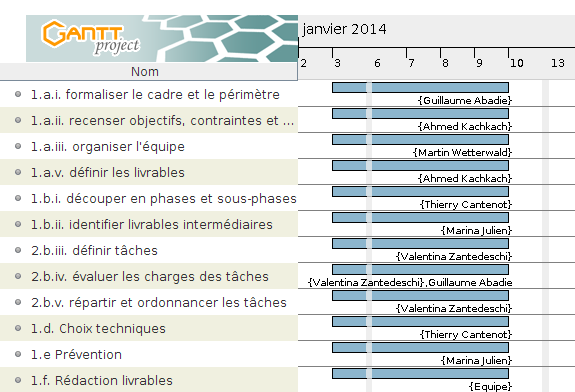
\includegraphics[scale=0.5]{images/SPIE_Init.png}
    \caption{Sous-phase d'initialisation}
    \label{diagram:si_map}
\end{figure}

\begin{figure}[h]
    \centering
    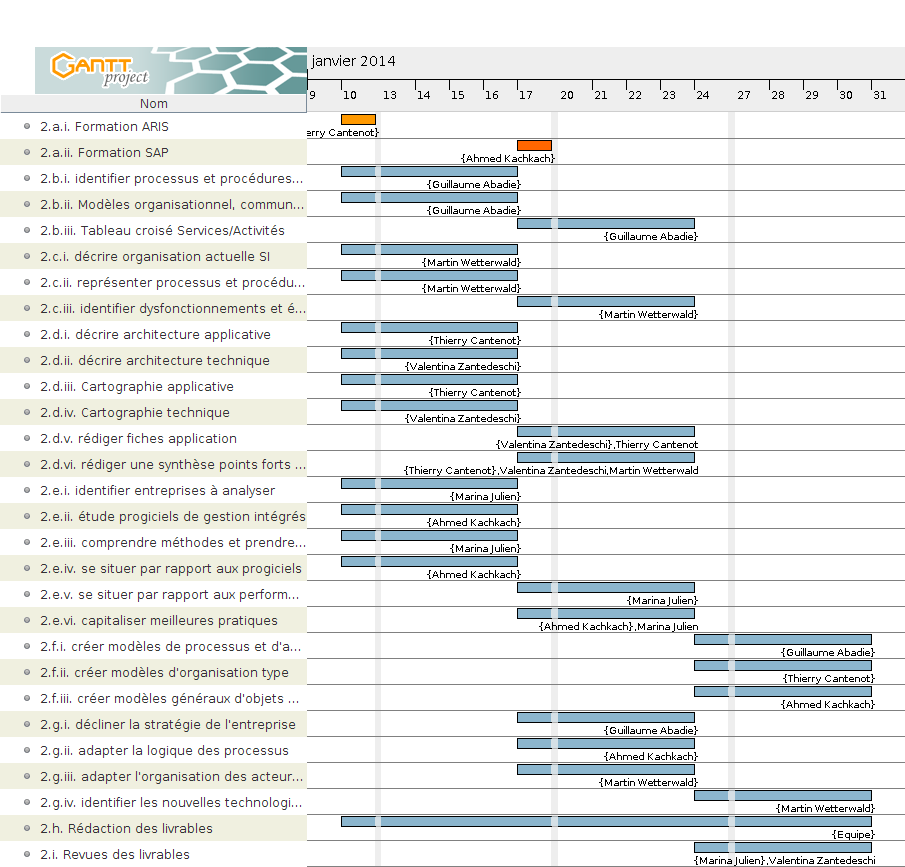
\includegraphics[width=100mm]{images/SPIE_besoins.png}
    \caption{Sous-phase d'expression des besoins}
    \label{diagram:si_map}
\end{figure}

\begin{figure}[h]
    \centering
    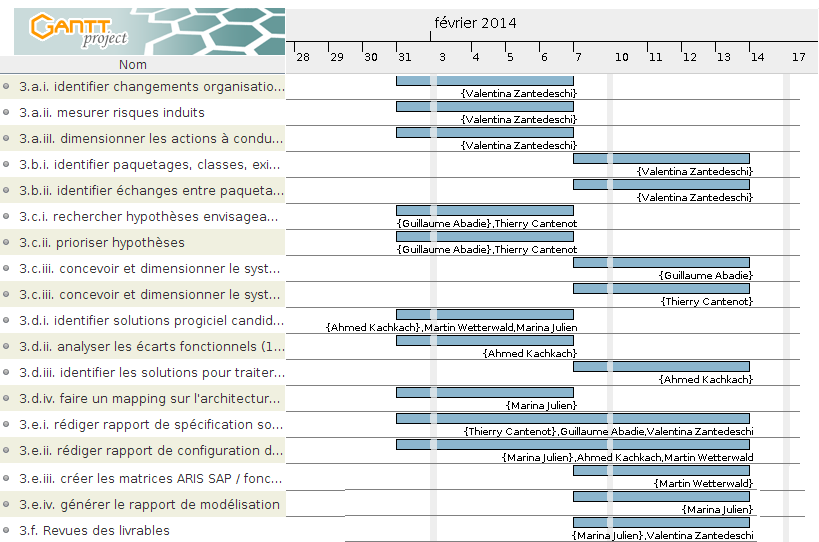
\includegraphics[width=150mm]{images/SPIE_3.png}
    \caption{Sous-phase de construction des solutions}
    \label{diagram:si_map}
\end{figure}

\begin{figure}[h]
    \centering
    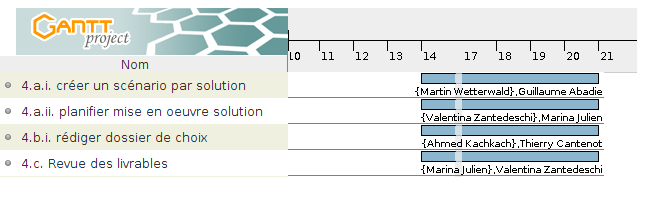
\includegraphics[scale=0.65]{images/SPIE_4.png}
    \caption{Sous-phase d'élaboration, évaluation et choix des scénarii}
    \label{diagram:si_map}
\end{figure}

\begin{figure}[h]
    \centering
    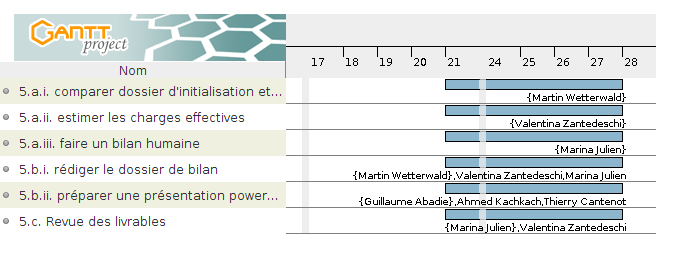
\includegraphics[scale=0.65]{images/SPIE_5.png}
    \caption{Sous-phase de bilan}
    \label{diagram:si_map}
\end{figure}

	\chapter*{Analyse des risques}
\addcontentsline{toc}{chapter}{Analyse des risques}
\chaptermark{Analyse des risques}

\subsection*{Méthodologie}
\addcontentsline{toc}{subsection}{Méthodologie}

Nous évaluons les risques de ce projet selon leur gravité et leur probablité. Les risques improbables et/ou à gravité mineure sont ainsi plus acceptables que ceux cumulant de fortes probabilités et gravités.

Les classes de probabilités que nous utilisons sont les suivantes:

\begin{itemize}
  \item \textbf{1}: Improbable 
  \item \textbf{2}: Rare
  \item \textbf{3}: Moyennement probable
  \item \textbf{4}: Probable
  \item \textbf{5}: Très probable
\end{itemize}

De même, les classes de gravité sont:

\begin{itemize}
  \item \textbf{1}: Mineure 
  \item \textbf{2}: Moyenne
  \item \textbf{3}: Majeure
  \item \textbf{4}: Critique
  \item \textbf{5}: Catastrophique
\end{itemize}

Nous choisissons donc les risques innacceptables (nécessitant une action) selon la matrice suivante:

\begin{tabular}{|c|l|l|l|l|l|}
     \hline
         P/G & \textbf{1} & \textbf{2} & \textbf{3} & \textbf{4} & \textbf{5}  \\ \hline
         \textbf{1} &   &   &   &   & x \\ \hline
         \textbf{2} &   &   &   & x & x \\ \hline
         \textbf{3} &   &   & x & x & x \\ \hline
         \textbf{4} &   & x & x & x & x \\ \hline
         \textbf{5} & x & x & x & x & x \\
     \hline
\end{tabular}

\newpage

\subsection*{Risques}
\addcontentsline{toc}{subsection}{Risques}

À partir de ces critères là, nous avons identifiés les risques suivants:

\begin{tabular}{|l||c|c|c|}
   \hline	
	   \textbf{Risque} & \textbf{Type} & \textbf{Probabilité} & \textbf{Gravité} \\ \hline \hline
	   Dépassement des échéances         & Organisation & 4 & 3  \\ \hline
	   Incohérence des livrables         & Organisation & 3 & 3  \\ \hline
  	 Absence d'un membre de l'équipe   & Organisation & 2 & 4  \\ \hline
	   Non respect des exigences         & Production   & 3 & 4  \\ \hline
	   Solution inadaptée                & Production   & 3 & 4  \\ \hline
	   Panne des outils de collaboration & Matériel     & 2 & 4  \\
   \hline
\end{tabular}

\subsection*{Plan d'action}
\addcontentsline{toc}{subsection}{Plan d'action}

Deux types d'actions peuvent être entreprises pour gérer ces risques:

\begin{itemize}
  \item \textbf{Actions de prévention}: diminuent la probabilité du risque
  \item \textbf{Actions de protection}: diminuent la gravité du risque
\end{itemize}

Voici donc notre plan d'action pour gérer les risques précédemment cités:

\begin{itemize}

  \item \textbf{Dépassement des échéances}
        \begin{itemize}
          \item \textbf{Prévention}: Établir un phasage précis, et une distribution équitable des tâches.
          \item \textbf{Protection}: Séparer les tâches en parties indépendantes pour ne pas ralentir toute l'équipe à cause du retard d'un des membres.
        \end{itemize}

  \item \textbf{Incohérence des livrables}
        \begin{itemize}
          \item \textbf{Prévention}: Effectuer un suivi qualité continu des livrables et réaliser des réunions pour faire une synthèse du travail de l'équipe.
        \end{itemize}

  \item \textbf{Absence d'un membre de l'équipe}
        \begin{itemize}
          \item \textbf{Prévention}: Dans le cas d'un imprévu (maladie, ...), les heures de travail râtées peuvent être récupérées en hors-horaire.
          \item \textbf{Protection}: Comme pour le premier risque, séparer les tâches et responsabilités en parties indépendantes (au possible).
        \end{itemize}


  \item \textbf{Non respect des exigences}
        \begin{itemize}
          \item \textbf{Prévention}: Établir une liste d'exigences précise à travers une étude métier détaillée et un receuil avancé des besoins du client (avec - si ambiguité - des réunions pour préciser ces derniers). Suivi de la complétion de ces exigeances tout au long du projet.
        \end{itemize}


  \item \textbf{Solution inadaptée}
        \begin{itemize}
          \item \textbf{Prévention}:  Assister à la formation ERP pour mieux appréhender ces solutions. Réaliser un receuil détaillé des besoins client (voir risque précédent). Étudier et rechercher les solutions existantes les mieux adaptées à ces besoins.
        \end{itemize}


  \item \textbf{Panne des outils de collaboration}
        \begin{itemize}
          \item \textbf{Prévention}: Choisir des outils dont l'infrastructure est robuste (haute disponibilité des serveurs).
          \item \textbf{Protection}: Constamment garder une copie locale du travail de l'équipe, en prévision d'indisponibilité des outils.
        \end{itemize}

\end{itemize}

% à finir 

	%\renewcommand{\chaptermark}[1]{\markboth{\MakeUppercase{#1}}{}}
	%\renewcommand{\sectionmark}[1]{\markright{#1}}

	%\addcontentsline{toc}{part}{Annexes}
	%\part*{Annexes}
	%\appendix
	%\include{implementationExercices}


    % ------------------------------------------------------------------- FOOTER
\end{document}
